%% thesis.tex 2014/04/11
%
% Based on sample files of unknown authorship.
%
% The Current Maintainer of this work is Paul Vojta.

\documentclass[masters]{ucbthesis}
\usepackage{biblatex}
\usepackage{wrapfig}
\usepackage{graphicx} %package to manage images
\usepackage{bbm}

% To compile this file, run "latex thesis", then "biber thesis"
% (or "bibtex thesis", if the output from latex asks for that instead),
% and then "latex thesis" (without the quotes in each case).

% Double spacing, if you want it.  Do not use for the final copy.
% \def\dsp{\def\baselinestretch{2.0}\large\normalsize}
% \dsp

% If the Grad. Division insists that the first paragraph of a section
% be indented (like the others), then include this line:
\usepackage{indentfirst}

\addtolength{\abovecaptionskip}{\baselineskip}

\newtheorem{theorem}{Jibberish}

\bibliography{references}

\hyphenation{mar-gin-al-ia}
\hyphenation{bra-va-do}

\begin{document}

% Declarations for Front Matter

\title{Can Satellites help First Responders in Ghana reduce Food Insecurity after Catastrophic Flooding? Laying the Foundations for a Double-Difference Impact Evaluation}
\author{Srilakshmi Ramesh}
\degreesemester{Spring}
\degreeyear{2021}
\degree{Master of Development Practice}
\chair{Professor Alain de Janvry}
\othermembers{Professor David Zilberman \\
  Professor David Wells Roland-Holst}
% For a co-chair who is subordinate to the \chair listed above
% \cochair{Professor Benedict Francis Pope}
% For two co-chairs of equal standing (do not use \chair with this one)
% \cochairs{Professor Richard Francis Sony}{Professor Benedict Francis Pope}
\numberofmembers{3}
% Previous degrees are no longer to be listed on the title page.
% \prevdegrees{B.A. (University of Northern South Dakota at Hoople) 1978 \\
%   M.S. (Ed's School of Quantum Mechanics and Muffler Repair) 1989}
\field{}
% Designated Emphasis -- this is optional, and rare
% \emphasis{Colloidal Telemetry}
% This is optional, and rare
% \jointinstitution{University of Western Maryland}
% This is optional (default is Berkeley)
% \campus{Berkeley}

% For a masters thesis, replace the above \documentclass line with
% \documentclass[masters]{ucbthesis}
% This affects the title and approval pages, which by default calls this
% document a "dissertation", not a "thesis".

\maketitle
% Delete (or comment out) the \approvalpage line for the final version.
% \approvalpage
%\copyrightpage

% % (This file is included by thesis.tex; you do not latex it by itself.)

\begin{abstract}

% The text of the abstract goes here.  If you need to use a \section
% command you will need to use \section*, \subsection*, etc. so that
% you don't get any numbering.  You probably won't be using any of
% these commands in the abstract anyway.

Invasive brag; forbearance.

\end{abstract}


\newpage\null\thispagestyle{empty}\newpage
\begin{frontmatter}

\begin{dedication}
\null\vfil
\begin{center}
To my family - Amma, Appa and Srisruthi - and to my my students in Sri Lanka, because of whom I study development practice, in pursuit of a desire to contribute to something much larger than myself.
\end{center}
\vfil\null
\end{dedication}

% You can delete the \clearpage lines if you don't want these to start on
% separate pages.

\tableofcontents
\clearpage
\listoffigures
\clearpage
\listoftables

\begin{acknowledgements}

In my view, the promise of impact evaluation lies in its ability to serve as a tool to hold us, as development practitioners, accountable to the vision of change we seek to achieve the world. I have sincere gratitude for several individuals at UC Berkeley, at Cloud to Street Public Benefit Corporation, in the Government of Ghana, and at the World Food Programme in Ghana for allowing me to practice this firsthand.\\

First, I am deeply indebted to the three members of my thesis committee, Professors Alain de Janvry, David Wells Roland-Holst, and David Zilberman, for their expertise and kindness in support of efforts to complete this study. I am also indebted to the program staff of the Development Practice Graduate Group; first, George Scharffenberger, a teacher and mentor of mine, for helping cultivate my skills in development practice, next, Lisa Robinson and Lauren Krupa, for their invaluable and consistent support over the two years of my graduate school journey, and last but not least, Professor Zilberman, not only for admitting me to the program two years ago, but for providing me with a community of development practitioners that has served me in immeasurable ways.\\

Next, I am immensely grateful to the entire team at Cloud to Street, PBC for their longstanding support of this work from its inception in May 2020. In particular, a sincere note of thanks to CEO Bessie Schwarz for her enthusiastic support of an impact evaluation, to Emmalina Glinskis for her leadership, time, and expertise in the fields of remote sensing and flood response in Ghana, to Max Goodman and Tyler Anderson for the same, and Dr. Elizabeth Tellman for her guidance that supported this study’s literature review. The Cloud to Street team gratuitously provided to me the full dataset used in this study. Without them, this work would have been wholly impossible.\\

Last but not least, I am deeply grateful for Charlotte Norman and Victor Abbador of the National Disaster Risk Management Organization in the Government of Ghana’s Ministry of Interior. Conversations with these individuals provided invaluable qualitative support for the findings in this study. I am also deeply grateful for John Sitor at WFP Ghana and Charlotte for their support in requisitioning the data required for this study.
\end{acknowledgements}

\end{frontmatter}

\pagestyle{headings}

% (Optional) \part{First Part}

\chapter{Acronyms}

Several acronyms are used in this paper. The following table lists all the acronyms used in this paper for reference.

\begin{table}
\centering
\begin{tabular}{|c|c|}
\hline
\textbf{Acronym} & \textbf{Expansion} \\
\hline
ATE & Average Treatment Effect \\
ESA & European Space Agency \\
CIESIN & Center for International Earth Science Information Network \\
FIS & Flood Information System \\ 
GADM  & Global Database of Administrative Areas \\
HRSL & High Resolution Settlement Layer \\
IFRC & International Federation of the Red Cross \\
LMIC & Low and Middle Income Countries \\
NADMO & National Disaster Risk Management Organization \\
NASA & National Aeronautics and Space Administration \\
OLS & Ordinary Least Squares \\
UN & United Nations \\
WFP & World Food Programme \\

\hline
\end{tabular}
\caption{All acronyms used in this paper}
\end{table}


\chapter{Introduction}

Across the African continent, not only is severe flooding becoming more frequent during the rainy season because of climate change, poorer individuals are overexposed to flooding relative to those who are not poor.\cite{douglas2008unjust} This poverty-climate nexus is growing in scale; a growing number of people experiencing poverty live in floodplains, largely due to their limited alternatives in terms of housing\cite{abubakari2019cities} (i.e. people with limited income who cannot afford housing in non flood-prone regions tend to settle within flood-prone areas, which tend to be cheaper).\cite{mensah2020causes}\\

In Ghana, frequent, catastrophic flooding affects millions of people every year. Recurring flood events in Accra, Kumasi, Tamale, Sekondi-Takoradi, Eastern and Volta regions claims hundreds of lives and destroys valuable assets worth thousands of Ghana cedis yearly.\cite{abubakari2019cities} The central government of Ghana, as a result, is incurring larger annual costs in post-flood disaster relief due to the increased frequency and severity of natural disasters nationwide.\\

A critical component of preparing for, responding to, and recovering from flood emergencies is information management.\footnote{The information in the rest of this section comes from more than 15 semi-structured interviews, and internal meetings held with senior NADMO disaster management officials between May and November 2020.} In order to effectively coordinate the logistics of a flood preparedness, response or recovery operation, first responders with the Ghanaian central government, as well as humanitarian relief organizations such as the IFRC and the UN WFP, require accurate, timely and disaggregated data on flooding. Such accurate, timely and disaggregated data includes flood damage estimates. Flood damage estimates include the number of flood-struck civilians, the length of flood-destroyed roads, and the area of flood-affected cropland in any given region. It also includes geospatial and climatological information, such as flood extents, precipitation data and rainfall levels.\\

Information on flood damage is required to quickly and accurately target humanitarian assistance in the event of a flood. The aid targeting process involves at least three unique tasks: 

\begin{itemize}
    \item disbursing the right type of aid,
    \item disbursing the right amount of aid, and
    \item identifying the right individuals to give aid to.
\end{itemize}

Optimizing these three aspects of aid targeting requires timely and accurate flood damage estimates across Ghana. Within the flood response ecosystem in Ghana, the status quo in terms of obtaining such information is that first responders primarily rely on sources of ‘ground truth’. The main sources of ground truth are reports on flooding in the media, civilian hotline information, and need assessments in which teams of first responders visit flood-affected areas to collect damage estimates. By relying primarily on ground truth, first responders in Ghana are often unable to respond to flood events fast enough.\\

One promising source of flood information that could represent an improvement upon this status quo is satellite imagery. Using remote sensing technology, one can leverage the imagery provided by public satellites that circle the earth to map floods, and thus better understand where flooding is taking place across the world. By overlaying flood maps with geospatial data on key assets - such as the locations of buildings, households and roads - one then has a powerful data-driven tool to improve policy-making around flood preparedness, response, and recovery in flood-prone communities. This satellite-based flood information is a critical component of the Government of Ghana’s plan for improving the country’s long-term flood preparedness, and building its overall resilience to climate change.\\

Satellite-based flood information has its advantages and disadvantages. The key advantage is that it enables first responders to identify flooded regions of the country in near-real time, and may provide more accurate estimates of flood-caused damage in quicker amounts of time relative to ground truth sources. However, the disadvantages of satellite-based flood information include that it does not provide insight into the extent or the nature of the damage. In pilot studies of satellite-based flood information systems, governments often opt to send in first responders to flooded regions in order to verify the accuracy of the satellite-based flood information they might receive from external data providers.\\

The next section outlines gaps in the  literature on the efficacy of satellite-based flood information in improving development outcomes.

\chapter{Literature Review}

Over the last 25 to 30 years, the explosive growth in computing power, data science, and technological advancement has created a market for data science products aimed specifically at transforming the decisions made by government policymakers everyday. These data science products come in one of many forms, from online dashboards, to interactive maps, to mobile applications. New trends in the public sector around ‘evidence-based’ or ‘data-driven’ decision making have expanded the market for data science products tenfold. In today’s world, policymakers have available to them a wide marketplace of data science products that claim to optimize, augment, and improve the efficacy, accuracy, efficiency, and speed of their decisions. However investing in these products comes at significant cost to governments; data science products, like all technology, are extremely expensive, usually require multi-year commitments from governments to install and roll out, and usually require significant cultural shifts in government agencies to embrace quantitative, data-driven modes of thinking.\\

Satellite-based flood information represents one example of a data science product that claims to optimize government decision making around emergency response. However, there is a dearth of literature on the efficacy of satellite-based flood information systems in actually improving observable development outcomes. The section outlines the two key pieces of literature that exist in this field, at the intersection of applied economics and remote sensing.\\

The first is a March 2018 paper by Oddo et. al.\cite{oddo2018socioeconomic} that provides an academic basis for a satellite-based flood information system developed for Ghana. The study integrates a socioeconomic damage assessment model with a near real-time flood remote sensing and decision support tool (NASA’s Project Mekong). Using the 2011 Southeast Asian flood as a case study, this tool is used to successfully derive flood-affected population, infrastructure and land cover estimates in the aftermath of this flood in the Mekong River Basin. Results of this study suggest that rapid initial estimates of flood impacts can provide valuable information to governments, international agencies, and disaster responders in the wake of extreme flood events. The second is a September 2019 study by Oddo et. al.\cite{oddo2019value} that points to the social and economic value of investing in satellite-based flood information systems. This study simulates a hypothetical flood event in Thailand, models vehicle routes and uses a value of information metric to quantify the social value and economic benefit of implementing a near-real-time flood impact system compared to ‘baseline routing strategies.’ Specifically, the study finds that the application of near real-time Earth observations can improve the response time and reduce potential encounters with flood hazards when compared with baseline routing strategies. Results indicate a potential significant economic benefit (i.e. millions of dollars) from applying near real-time Earth observations for improved flood disaster response and management.\\

In sum, both of these studies show promise that satellite-based flood information generates positive returns for policymakers. However, neither of these studies look at the relationship between satellites and food-based aid, and neither look at causation with respect to the impact of satellites on development outcomes. In terms of the relationship between satellites and development outcomes, the closest related work is the ongoing research study by Josh Blumenstock at UC Berkeley that examines the use of satellite imagery in optimizing aid targeting (i.e. cash-based transfers) in Togo\cite{blumenstocktogo}. This study however also does not examine the impact of satellites on improving food security outcomes, it only looks at using satellites to optimize cash-based transfers.\\

All in all, generating quasi-experimental evidence around the efficacy of satellite-based flood information platforms in improving community-level development outcomes would add valuable context to the conclusions derived from these prior studies, which do not use experimental or quasi-experimental methods. Understanding the impact of satellite-based flood information in development outcomes would provide insight into the ability of this technology to support climate resilience amongst flood-prone communities, and build the capacity of government policymakers to in turn strengthen the long-term flood preparedness of these communities. 

\chapter{Program Description}

This section provides an overview of the program and anecdotal, out-of-country evidence of the value of the program based on anecdotal evidence provided by NADMO.\footnote{All of the information in this section comes from more than 15 semi-structured interviews, and internal meetings held with senior NADMO disaster management officials between May and November 2020.}

\section{Overview}

The program in question in this study is a satellite-based Flood Information System or FIS, which was provided to NADMO, the Government of Ghana’s foremost agency for disaster risk management that is housed in the Ministry of Interior. Private data providers with expertise in the discipline of aggregating data from satellites, also known as remote sensing, have specialized in the development and sale of FIS platforms particularly for emergency response in LMICs. In August 2018, one such data provider, Cloud to Street, developed and implemented a FIS to augment NADMO's capabilities around flood preparedness, response, and recovery. For the last three years, Cloud to Street has provided NADMO with the FIS platform in an effort to optimize these three processes, at the request of the central government.\\

The FIS that Cloud to Street implemented for NADMO in 2018 is currently the Government of Ghana’s largest repository of flood information to-date. The FIS leverages public satellites to map floodplains and near-real time flood events. The platform itself has two main components:
\begin{enumerate}
  \item A 35-year annualized historical record of flood frequency data.
  \item Weekly, near-real time earth observations of ongoing flooding during Ghana’s rainy season (August to December of each year).
\end{enumerate}

As part of the near-real time monitoring service, the FIS has provided NADMO disaster management officials with quantifiable flood damage estimates as flooding is taking place. These estimates include the total number of people affected by flooding, the total area of flooded cropland, and the total number of schools affected by flooding in each district of Ghana each week. This information comes by way of an interactive dashboard, interactive maps, and downloadable files in machine-readable formats. Key flood alerts are provided to district-level NADMO officers via Whatsapp as well.\\

Since the program’s inception in August 2018, NADMO officials have used it to acquire near-real-time flood damage estimates to target humanitarian aid both faster, and more accurately. Anecdotally, NADMO officials report that they hope to use the FIS to augment its capabilities around anticipating floods prior to the flood striking. Achieving these objectives will enable NADMO to reduce the agency’s overall response time to flood events, and in turn, reduce the recovery time it takes flood-struck communities to bounce back. Response measures might include the time taken to preposition and disburse aid post-flooding, and recovery measures might include the time taken for individuals to recover lost wealth, and for farmers to resume farming activities.\\

The FIS has been operational in Ghana under the management of NADMO for 3 years: 2018, 2019, and 2020. In 2018, the FIS was launched as a pilot program for NADMO in collaboration with the African Risk Capacity, which is a division of the African Union. In 2019, NADMO launched a second pilot to further test the FIS capabilities. The first two pilot years were used to validate FIS information against ground truth estimates to evaluate its accuracy and implement functional improvements. In 2020, NADMO entered its first full, non-pilot year of FIS operations. That year, NADMO held a few agency-wide trainings on how to use the FIS to inform flood response operations. FIS information was purportedly disseminated to NADMO district officers to support district-level flood preparedness and response activities throughout the 2020 rainy season. With the end of the most recent rainy season in December 2020, NADMO concluded its use of the FIS. The agency plans to renew usage of the FIS for the 2021 rainy season.\\

The program start and end dates are summarized as follows:
\begin{itemize}
  \item Program start date: August 2018
  \item Program end date: December 2020
\end{itemize}

\section{Out-of-country anecdotal evidence of program value}

From May to November 2020, emergency management officials in the Republic of Congo were also interviewed to collect qualitative, anecdotal evidence on the value provided by a satellite-based FIS that their government had purchased in 2018. The first responders in the Congo reported that they were able to use the FIS to optimize aid targeting operations, such as where to target cash-based transfers. Implementing cash transfers requires a district to have functioning markets. The FIS provided the first responders with the location of functioning and flood-damaged markets, which they used to disburse cash-based and food-based assistance, respectively. According to these interviewees, the FIS information enabled these first responders to reach over 180,000 flood-affected Congolese civilians over the 9 months of the program’s operation.\\

In sum, the program description illustrates a potentially positive return on investment in the FIS. By using the FIS, NADMO officials might reduce (and thereby, improve) their agency-wide 'response time' to flooding across the country during the 2020 rainy season. If true, this in turn might engender reduced (and improved) bounce-back time for flood-prone districts in Ghana, where 'bounce back' might be measured in terms of food security.








\chapter{Study Hypothesis}

The study hypothesis is that the FIS reduces food insecurity in high flood-risk Ghanaian districts relative to low-flood risk Ghanaian districts.\footnote{All of the information in this section comes from more than 15 semi-structured interviews, and internal meetings held with senior NADMO disaster management officials between May and November 2020.}\\

Taking a closer look at the nature of the FIS as a program, we see why this hypothesis makes sense. One of the main purposes of the FIS is to provide NADMO with the information it needs to optimize aid targeting decisions. These decisions can be described as the type, amount, and location of aid to provide after a flood has taken place. Next, one of the main forms of aid that NADMO provides is food aid. NADMO officers are interested in the appropriate placement of food aid in flood-prone regions. After flooding has taken place, food aid would be more readily available to those that need it most. This might have the effect of reducing the recovery time of these communities after flooding, according to NADMO officials.\\

As an additional point of evidence around the significance of food aid, NADMO’s partnership with UN WFP is what enables NADMO to use the FIS. WFP Ghana has provided NADMO with the funds to purchase the FIS via contract with Cloud to Street for the last three years. In sum, we see that a measure of food security at the household or district level would be an ideal outcome variable to examine programmatic impact.\\

One would also expect the benefits of the FIS to be most prevalent in the districts of Ghana that are at highest flood risk relative to those that are not at flood risk. This is because by leveraging satellites, the FIS provides a flood preparedness platform that promises to enable NADMO with the information they need to reduce the harm caused by flooding in the districts that are routinely hit the hardest. The flood frequency maps and near-real time flood damage estimates contained in the FIS are meant for NADMO to use in order to optimize its aid targeting activities. Anecdotally, NADMO officials report that they plan to use the FIS to determine the appropriate type and quantity of both food and cash-based aid for each district affected by flooding.


\chapter{Data}

This section outlines four components: the two main types of data used in this study, how the geospatial data layers were overlaid to determine units of ‘population affected’ and ‘cropland affected’ by flooding, as well as the metadata for all data sets. All data used in this study was provided gratuitously by Cloud to Street, a remote sensing startup that specializes in the development and sale of satellite-based flood information systems for emergency management in LMICs.\\

Two main types of data were used in this study:

\begin{enumerate}
  \item Flood recurrence intervals; and
  \item Flood damage estimates.
\end{enumerate}

The flood recurrence intervals data contains information about how frequently it floods in each district of Ghana each year. Flood frequency data was available for this study in the form of satellite imagery. These images can illustrate how often a given district of Ghana floods each year. Using flood frequency satellite data was one of the two key components involved in developing the Flood Risk Index. The flood damage estimates data contains information about the point or areal location of critical assets in each district in Ghana. Flood damage estimates were also available for this study in the form of satellite imagery. These estimates - when overlaid onto the flood frequency satellite imagery - provide an adequate measure of flood risk, by revealing which districts in Ghana both flood the most frequently and contain the largest number of flood-risk assets.\\

Each of the two data types above were used in this study in the form of annualized, district-level observations. This is because of the study hypothesis that the program’s benefits are most clear in flood-prone districts relative to non-flood prone districts. Each data type is detailed in the section below.

\section{Flood recurrence intervals}

Flood frequency is often measured using flood recurrence intervals. A flood’s ‘recurrence interval’ is the probability that a flood will occur in any given year. It essentially provides an estimated interval of time between floods of comparable size or severity. If a flood has a recurrence interval of 100 years, for example, the probability of its occurrence in any given year - also known as its annual exceedance probability - is 1/100 or 0.01. If a flood has a recurrence interval of 5 or 2 years, for example, its annual exceedance probability is much higher than this, respectively 1/5 or 1/2 (20 percent or 50 percent). In sum, it is possible to use recurrence intervals to map the extent to which each of Ghana’s 216 districts are flood-prone. Flood frequency maps for each return period can be generated with the following steps:

\begin{enumerate}
  \item Water detection algorithms take an input of satellite image and flagged each pixel on the image as either a flooded pixel or not flooded pixel (1 or 0). These algorithms ultimately provide a layer of individual water extents for the region in the satellite image. To measure flood frequency, satellite imagery was pulled from two public satellites that provide high-resolution data: Landsat, which provides 30-m resolution imagery, and MODIS, which provides 250-m resolution imagery.

  \item These individual flood extents are then aggregated such that the maximum flood extent is taken for each pixel, each year. Each of these years correspond to a flood recurrence interval.
  
  \item The annual maximum flood extents per pixel are used to calculate the annual probability of a given pixel flooding. These annual probabilities of a given pixel flooding are then aggregated to a given unit of aggregation (e.g. the GADM Administrative Level 2 in Ghana), and can provide the annual probability of a given district in Ghana flooding.
  
  \item These annual probabilities of a given district flooding are converted to recurrence intervals in years.
\end{enumerate}

It is possible for a water detection algorithm to mistake seasonal water, which is water that is present in a pixel every year at the same time and permanent water bodies - like a lake, or a river - for a flood event. To account for this, the flood recurrence interval maps produced in Step 4 are cleaned to separate or mask out seasonal water and permanent water bodies using a separate data source that provides the location of such entities in Ghana.  The resulting map is then cleaned using a quality control check that results in the final historical flood frequency layers for each recurrence interval.

\subsection{Why using flood recurrence intervals makes sense to measure flood risk}

Research from the University of Bristol\footnote{In this study, the forecasting model used was provided by Fathom Global Flood Model (GFM, Sampson et al., 2015\cite{sampson2015high}) using the hydrodynamic model LISFLOOD-FP (Neal et al., 2012) and the MERIT Digital Elevation Models (DEM) derived river network (Yamazaki et al., 2019\cite{yamazaki2019merit})} shows that using maps of remotely-sensed flood recurrence intervals as described here is a good way to measure flood frequency - one the two key components of flood risk - if one is interested in measuring high-frequency flooding. The University of Bristol examined the consistency between flood recurrence maps and flood forecasting models using four large river basins across Africa. The analysis compared simulated flood expectation to the remotely sensed flood map for each pixel. The results show that at lower recurrence intervals (i.e. about 50 years), the remotely-sensed flood maps were more accurate than the forecasting model simulations. At higher recurrence intervals (i.e. about 100 years), the forecasting models are more accurate than the remotely-sensed flood maps.\\

Table 6.1 provides the five recurrence intervals used to develop the final Flood Risk Index: 2-year, 5-year, 10-year, 15-year, and 20-year. Recurrence intervals are provided in the column 'T'. 'Frequency' describes the flood frequency that each recurrence interval represents.

\begin{table}
\centering
\begin{tabular}{|c|c|p{10cm}|}
\hline
\textbf{T} & \textbf{Frequency} & \textbf{Interpretation}\\
\hline
2\rule{0pt}{4ex} & Very Frequent & Flags districts that have a 50 percent chance of flooding in the next year based on a ~35-year historical record. \\
5\rule{0pt}{4ex} & Frequent & Flags districts that have a 20 percent chance of flooding in the next year based on a ~35-year historical record. \\
10\rule{0pt}{4ex} & Moderately Frequent & Flags districts that have a 10 percent chance of flooding in the next year based on a ~35-year historical  record. \\
15\rule{0pt}{4ex} & Somewhat Frequent & Flags districts that have a 6.67 percent chance of flooding in the next year based on a ~35-year historical  record. \\
20\rule{0pt}{4ex} & Less Frequent & Flags districts that have a 5 percent chance of flooding in the next year based on a ~35-year historical record.\\
\hline
\end{tabular}
\caption{Recurrence intervals used in the Flood Risk Index}
\end{table}

\subsection{Recurrence intervals as flood frequency scenarios}

This section provides more intuition behind why recurrence intervals can be thought of as representing unique flood-frequency scenarios. Using satellites, we can use a flood’s recurrence interval to determine which of Ghana’s 216 districts are ‘very frequently’ flooded vs. ‘less frequently’ flooded.\\

The satellite-derived population impact estimates for Ghana’s 216 districts are shown in Table 6.2. This table contains sample rows of the recurrence interval data (which comes directly from satellites), along with the population estimates that is overlaid on the recurrence data. The ‘District’ column in this table refers to the name of the district in Ghana, corresponding to the GADM Administrative Level 2 region of Ghana. Each recurrence interval column corresponds to a unique flood-frequency scenario. Specifically, the ‘2-Year’ column gives the total number of flood-affected people residing in a given district given that this district is ‘very frequently flooded.’ Similarly, the ‘5-Year’ column provides the same data given that this district is ‘frequently flooded’. A full crosswalk of which recurrence intervals correspond to which flood-frequency scenarios is provided in Table 2. Numbers are in the 1000s.\\

\begin{table}
\centering
\begin{tabular}{|c|c|c|c|c|c|}
\hline
\textbf{District} & \textbf{2-Year} & \textbf{5-Year} & \textbf{10-Year} & \textbf{15-Year} & \textbf{20-Year}\\
\hline
Accra Metropolis\rule{0pt}{4ex} & 41 & 356 & 807 & 1071 & 1256 \\
Ada East\rule{0pt}{4ex} & 0 & 80 & 230 & 328 & 410 \\
Ada West\rule{0pt}{4ex} & 18 & 384 & 658 & 801 & 989 \\
Adaklu\rule{0pt}{4ex} & 0 & 0 & 0 & 0 & 0 \\
\hline
\end{tabular}
\caption{Sample of satellite-derived population impact estimates per flood-frequency scenario}
\end{table}

The 2-Year recurrence interval represents one extreme scenario: the most frequently flooded, which is termed the ‘Very Frequently Flooded’ scenario. The ‘20-Year’ recurrence interval represents the other extreme scenario: the least frequently flooded, which is termed the ‘Less Frequently Flooded’ scenario. We can determine the number of flood-affected people under each scenario as part of our measure of the overall flood risk:

\begin{equation}
Severity = Indicator * Population
\end{equation}

In this equation, 'Severity' represents the impact severity, which is either the number of flood-affected people or the acres of flood-affected cropland in a given recurrence interval. 'Indicator' refers to a boolean value 1 or 0 indicating whether the water detection algorithms detect that the collection of pixels that correspond to a given district are flooded or not in a given recurrence interval. 'Population' is the population of that district per HRSL data at that time.\\

\begin{table}
\centering
\begin{tabular}{|c|c|c|p{7cm}|}
\hline
\textbf{District} & \textbf{T} & \textbf{Impact Severity} & \textbf{Interpretation}\\
\hline
Ada East\rule{0pt}{4ex} & 2 & 0 * (Unknown value) = 0 & 0 people would be impacted by flooding in Ada East under the scenario that Ada East is a ‘very frequently’ flooded district \\
Ada East\rule{0pt}{4ex} & 5 & 1 * 80 = 80 & 80,000 people would be impacted by flooding in Ada East under the scenario that Ada East is a ‘frequently’ flooded district \\
\hline
\end{tabular}
\caption{Implementation of severity equation for Ada East district, flooded population estimate per recurrence interval}
\end{table}

Take for example, the district Ada East. If the water detection algorithms determine that Ada East is flooded in a given flood frequency scenario (e.g. the 2-Year Recurrence Interval flood frequency scenario), the boolean indicator becomes a 1. Table 6.3 implements the equation above to arrive at the estimated number of people that would be impacted by flooding under each flood-frequency scenario. We can interpret this as the following:

\begin{enumerate}
  \item Ada East is not a ‘very frequently’ flooded district, because the indicator in the 2-Year Recurrence Interval is 0.
  \item However, Ada East is a ‘frequently’ flooded district, because the indicator in the 5-Year Recurrence Interval is 1.
\end{enumerate}

This example illustrates how recurrence intervals correspond to flood-frequency scenarios. In sum, the gradient of flood-frequency scenarios helps determine which districts are more often flooded relative to the other districts.

\subsection{Satellite data sources used}

Four satellites provided all of the flood inundation data used by the water detection algorithms to map floods as part of the flood recurrence interval data. These sensors were the following:

\begin{enumerate}
  \item NASA Landsat 7,
  \item NASA Landsat 8,
  \item ESA Sentinel-1, and
  \item ESA Sentinel-2.
\end{enumerate}

Landsat 7 is the seventh satellite of NASA’s Landsat program. Launched on April 15, 1999, the primary objective of Landsat 7 is to update the global archive of satellite photos in order to provide recent, cloud-free images of Planet Earth.\cite{landsat} The Landsat 7 program is managed by the US Geological Survey. Landsat 8 is the most recently launched satellite in the Landsat program and was launched on February 11, 2013.\\

Sentinel 1 is the first in the Sentinel series of the European Union’s Copernicus program. According to the ESA\cite{sentinel1}, Sentinel-1 carries an advanced radar instrument to provide an all-weather, day-and-night supply of imagery of Earth’s surface. The ESA also describes Sentinel-2\cite{sentinel2} as a European wide-swath, high-resolution, multi-spectral imaging mission. This satellite is designed to give a high revisit frequency of 5 days at the Equator, because of which high-resolution data from Sentinel-2 can support the change detection of flood events for affected countries. Open-source platforms for remote sensing like Google Earth Engine have enabled remote sensing scientists to use the imagery from these four sensors to map floods in near-real time in many low and middle income countries, like Ghana.

\section{Flood damage estimates}

Flood return periods only address one of the two components of flood risk: flood frequency. The second dimension is social and economic vulnerability. This can be measured using the spatial distribution of households and buildings, agricultural land, and other assets of interest. The intersection of these two layers of satellite imagery - a map of flood frequency, and a map of critical assets - provides a more complete measure of flood risk than either layer of imagery used independently. Two types of critical assets were used in this study:\\

\begin{itemize}
  \item flood-affected population, and
  \item flood-affected cropland.
\end{itemize}

Each of these assets is described below.

\subsection{Flood-affected population}

The population data used was the total number of flood-affected populations in each of Ghana’s districts. This data was based on the HRSL\cite{hrsl}. The HRSL is a free, open-source gridded product that provides estimates of populations by combining high-resolution satellite imagery and local census data at 30-meter resolution.\\

Facebook and Columbia university have collaborated to publish the HRSL repository. The Connectivity Lab at Facebook used 0.5 meter DigitalGlobe satellite imagery and machine learning to create pixel based settlement extents at 30 meters. CIESIN then aggregated and distributed the population count from census data to the pixel based settlement extents. HRSL data is currently available in over 100 countries (Facebook, 2017).

\subsection{Flood-affected cropland}

The cropland data was sourced from Clark University’s Mapping Africa Project\cite{mappingafrica}. The cropland data used was the total sq. km. of flood-affected cropland in each of Ghana’s districts. high resolution cropland data at 3-meters. The Mapping Africa Project uses both traditional mapping of cropland with machine learning to improve the classification of agricultural cropland across the African continent.

\section{Overlaying geospatial layers of flood recurrence data and flood damage estimates}

To arrive at the final flood-affected cropland and flood-affected population impacts, the cropland and population datasets are overlaid on the flood layers to determine which pixels in each layer intersect with one another. This intersection comes in the form of a raster layer, that contains only the areas of the country where cropland or population were ‘impacted’ by flooding. This intersection layer, which is at the pixel level, is then aggregated to the administrative unit of interest to arrive at the total number of square kilometers of flood-affected people or cropland per administrative unit, respectively. In this study, the administrative unit of interest was the district-level (i.e. GADM Administrative Level 2).

\section{Metadata}

Using the techniques described in Section 6.3, Cloud to Street’s remote sensing scientists provided tidy datasets of flood impact used throughout this study. This data was used without modification for the purposes of this study. The specifications (or metadata) for each dataset received from Cloud to Street can be seen in the table below.

Cloud to Street provided a variety of datasets that provide a wealth of satellite-driven estimates of population and cropland impacted by flooding overtime at the district level in Ghana. Each row in each of the datasets provided by Cloud to Street corresponded to each district in Ghana (i.e. GADM Level 2) The majority of this data is available open-source on the Cloud to Street website.

\begin{table}
\centering
\begin{tabular}{|p{4cm}|p{2cm}|p{8cm}|}
\hline
\textbf{Dataset Name} & \textbf{No. of datasets} & \textbf{Description}\\
\hline
Flood impact in 2-year interval & 3 & Number of flood-affected people per district, and Hectares of flood-affected cropland per district\\
Flood impact in 5-year interval & 3 & Same as above for 5-year  interval\\
Flood impact in 10-year interval & 3 & Same as above for 10-year  interval\\
Flood impact in 15-year interval & 3 & Same as above for 15-year  interval\\
Flood impact in 20-year interval & 3 & Same as above for 20-year  interval\\
Annualized, district-level flood damage estimates & 1 & Annualized impacts for total flood-affected cropland, total flooded area, and total flood-affected population per district (216 districts total)\\
\hline
\end{tabular}
\caption{Metadata}
\end{table}

Cloud to Street provided a variety of datasets that provide a wealth of satellite-driven estimates of population and cropland impacted by flooding overtime at the district level in Ghana. Each row in each of the datasets provided by Cloud to Street corresponded to each district in Ghana (i.e. GADM Level 2) The majority of this data is available open-source on the Cloud to Street website.\cite{cloudtostreet}

\chapter{External and Internal Validity}

The following discusses the methods used to establish external and internal validity in the study.\\

\section{External Validity}

Impact evaluations ideally employ both random selection and random assignment to establish external validity and internal validity, respectively. Because it is usually not possible to include the entire target population in the evaluation sample, random selection is often used to draw an evaluation sample from the target population.\\

In this study, however, it was possible to include the entire target population in the evaluation sample thanks to the rich repository of remotely-sensed flood information available for the analyses. Both the target population and the evaluation sample for this study is all 216 districts of Ghana. This means that inferences from the impact evaluation would apply directly to the target population of all districts in Ghana so long as internal validity is established.

\section{Internal Validity}

Internal validity in a study that involves causal inference such as this one is best ensured by using random assignment. This means that each sampling unit in the evaluation sample is randomly assigned to one of two groups: the treatment group, which receives the program, and the control group, which does not receive the program. Random assignment is the gold standard of causal inference; when randomization is successful, it ensures that observed differences between the treatment and control groups are an unbiased estimate of the average treatment effect within the evaluation sample.\\

A randomized evaluation could not be done for the program in question because the program could not be randomly assigned to the 216 Ghanaian districts in the evaluation sample. Specifically, the FIS was housed at the NADMO headquarters in Accra, and NADMO officials in Accra used the FIS to coordinate district-level aid distribution efforts on a periodic basis.\\

Where random assignment of the program is not feasible, one might look for a natural experiment instead.  One option is to use a double difference evaluation to draw causal inferences if the identifying assumption of parallel trends is satisfied. In a double difference evaluation, one compares average values of a given outcome variable of interest between a group that receives the treatment, and the group that does both before and after the introduction of the program. The double difference design accounts for the ‘before/after’ comparison and the ‘with program/without program’ comparison. The before/after and with/without scenarios for this study are summarized in Table 7.1.\\

\begin{table}
\centering
\begin{tabular}{|c|c|}
\hline
\textbf{Study design component} & \textbf{Description}\\
\hline
Before\rule{0pt}{4ex} & Before August 2018 \\
After\rule{0pt}{4ex} & After December 2020 \\
With\rule{0pt}{4ex} & Flood-prone districts of Ghana \\
Without\rule{0pt}{4ex} & Non flood-prone districts of Ghana \\
\hline
\end{tabular}
\caption{Study design components}
\end{table}

As shown in Table 7.1, the before-after comparison in this study is the time prior to August 2018 and the time after December 2020 respectively. The with-without comparison in this study is done using flood-prone districts of Ghana as the ‘with’ group and the non flood-prone districts of Ghana as the ‘without’ group.\\

The next section outlines all components of this study’s double difference evaluation.

\chapter{Methods}

In a double difference evaluation, the first step is to assign sampling units to treatment and control groups based on given measurable criteria. After sampling units have been assigned to treatment and control groups, the control group serves as a valid counterfactual for the treatment group if and only if one can establish parallel trends between the treatment and control group on the outcome variables of interest. Satisfying the assumption of parallel trends is how one ensures internal validity in a double difference evaluation and what ensures that the  double difference estimator serves as an unbiased estimate of the average treatment effect.\\

The measurable criteria used in this study was a district-level Flood Risk Index calculated using remotely-sensed flood frequency and flood impact information. Flood risk was used to group districts into treatment and control groups based on the study hypothesis, which details why the benefits of the FIS might be most salient in flood-prone districts relative to non flood-prone districts. The steps to estimate impact were as follows:

\begin{enumerate}
  \item Develop a Flood Risk Index.
  \item Threshold the Flood Risk Index.
  \item Examine parallel trends between treatment and control groups on the outcome variables.
\end{enumerate}

Each step is detailed below.

\section{Develop a Flood Risk Index}

Measuring flood risk is a complex process; it involves accounting for not only a given region’s flood frequency but also the region’s social and economic vulnerability. If a given region has many low-rise buildings or farmable land on it, for example, it is at higher flood risk than a comparable region without those assets on it. It is possible to capture both important dimensions of flood risk using two types of geospatial information: flood recurrence intervals, and the location of various assets of interest (e.g. people, cropland, roads). The intersection of these two types of flood information for various intervals of time provides a more complete measure of flood risk that is based not only on flood frequency, but the overall historical flood impact as well. The flood risk index calculation methodology is as follows:

\begin{enumerate}
  \item Compute the average number of flood-affected people per year per district.
  \item Compute the average area of flood-affected cropland per year per district.
  \item Convert the average area of flood-affected cropland per year per district into average numbers of flood-affected people per year per district.
  \item Sum the values from Steps 1 and 3 to calculate the raw Flood Risk Index.
  \item Use a z-score conversion to normalize the raw Flood Risk Index values.
\end{enumerate}

Each of these steps is detailed further below.

\subsection{Compute the average number of flood-affected people per year per district.}

Given that recurrence intervals can be thought of as different flood frequency scenarios, we can use the data from Table 6.2 to calculate the average number of flood-affected people overall flood frequency scenarios. We can do this by calculating the marginal number of flood-affected people under each scenario:

\[ MI_T = (I_T - I_{T-1}) / T \]

Where (\({MI_T}\)) is the marginal impact under recurrence interval (\({T}\)). The term (\({I_T}\)) represents the total impact (i.e. total number of flood-affected people) and (\(I_{T-1}\)) represents the same for the prior recurrence interval. Table 8.1 uses the values from Table 6.2 to calculate the marginal impact under each recurrence interval for the Ada East district. Table 8.1 illustrates how one would implement the equation on the last page to calculates the marginal population impact for each district across all five recurrence intervals.\\

Finally, we can calculate the average impact across all flood frequency scenarios by applying a weighted sum, like so:

\[ I_{\mu} = \sum_{T=1}^{5} MI_T * w_T \]

In this equation, the left-hand term refers to the average population impact or the average cropland impact in a given district across all flood recurrence intervals. The term \({MI_T}\) represents the marginal impact in a given recurrence interval \({T}\). The term \({w_T}\) represents the weight for a given recurrence interval as shown in Table 8.2. Weights provided in Table 8.2 correspond roughly to the recurrence interval's annual exceedance probability (e.g. 2-Year Recurrence Interval corresponds to a 50 percent probability of occurrence, 5-Year Recurrence Interval corresponds to a 20 percent probability of occurrence, and so on). All weights in Table 8.2 sum to 1.00.\\

Table 8.3 provides an example of how the formula from the prior page, used to calculate average impact, is implemented. As shown in Table 8.3, the computed population impact for the Ada East district is 5.36231. This computed average is a measure of both flood frequency and impact severity. It measures not only the frequency of flooding in a given region, but the total number of people that would be affected if that region were to actually flood in the following year. \\

\begin{table}
\centering
\begin{tabular}{|p{3cm}|c|c|}
\hline
\textbf{Interval (\({T}\))} & \textbf{District} & \textbf{Marginal Population Impact}\\
\hline
2-Year Interval\rule{0pt}{4ex} & Ada East & (0 - 0) / 2 = 0 \\
5-Year Interval\rule{0pt}{4ex} & Ada East & (80 - 0) / 5 = 16 \\
10-Year Interval\rule{0pt}{4ex} & Ada East & (230 - 80) / 10 = 15\\
15-Year Interval\rule{0pt}{4ex} & Ada East & (328 - 230) / 15 = 6.533\\
20-Year Interval\rule{0pt}{4ex} & Ada East & (410 - 328) / 20 = 4.1\\
\hline
\end{tabular}
\caption{Marginal population impact for Ada East}
\end{table}

\begin{table}
\centering
\begin{tabular}{|c|c|}
\hline
\textbf{Recurrence Interval (\({T}\))} & \textbf{Weight (\({w_T}\))}\\
\hline
2-Year Interval\rule{0pt}{4ex} & 0.580 \\
5-Year Interval\rule{0pt}{4ex} & 0.200 \\
10-Year Interval\rule{0pt}{4ex} & 0.100 \\
15-Year Interval\rule{0pt}{4ex} & 0.07 \\
20-Year Interval\rule{0pt}{4ex} & 0.05 \\
\hline
\end{tabular}
\caption{Weights for each Recurrence Interval}
\end{table}

\begin{table}
\centering
\begin{tabular}{|p{4cm}|p{7cm}|}
\hline
\textbf{Metric} & \textbf{Formula}\\
\hline
Avg Flood-Affected Population (\({I_P}\)) & (0 * 0.58) + (16 * 0.20) + (15 * 0.10) + (6.533 * 0.07) + (4.1 * 0.05) = 5.36231\\
\hline
\end{tabular}
\caption{Average Population Impact for Ada East}
\end{table}

We now repeat this step using cropland data, and calculate the average hectares of flood-affected cropland per district.

\subsection{Compute the average area of flood-affected cropland per year per district.}

\begin{table}
\centering
\begin{tabular}{|p{3.5cm}|p{4.5cm}|p{4.5cm}|}
\hline
\textbf{District} & \textbf{Avg Flood-Affected Population (\({I_P}\))} & \textbf{Avg Flood-Affected Cropland}\\
\hline
Accra Metropolis\rule{0pt}{4ex} & 30.744500 & 0.000025\\
Ada East\rule{0pt}{4ex} & 5.36231 & 0.214428\\
Ada West\rule{0pt}{4ex} & 23.737333 & 0.725215\\
Adaklu\rule{0pt}{4ex} & 0.000000 & 0.000772\\
\hline
\end{tabular}
\caption{Average overall annual flood impacts per district, inconsistent units of measurement}
\end{table}

Using the process outlined in Step 1, we calculate the average hectares of flood-affected cropland for each of Ghana's 216 districts. A sample of the full results of implementing this calculation is provided in Table 8.4. As shown in Table 8.4, the average overall annual flood impacts per district is simply a weighted sum of the marginal population impacts.

\subsection{Convert the average area of flood-affected cropland per year per district into average numbers of flood-affected people per year per district.}

We cannot yet add the values from Steps 1 and 2 together, because the two assets are not in the same unit of measurement. From Step 1, we see that the unit of the people-based asset is the number of flood-affected people per district. From Step 2, we see that the unit of the cropland-based asset is the area of flood-affected cropland per district.\\

To ensure these two assets are comparable, we can set an arbitrary conversion rate to convert the cropland-based asset into the people-based one (i.e. convert the average area of flood-affected cropland into an average number of flood-affected people). For the purposes of this study, the following conversion rate is used:

\[ 10{H} = 1{P} \]

In this equation, \({H}\) represents the hectares of flood-affected cropland, and \({P}\) represents the number of flood-affected people. The conversion rate used is 10 hectares of flood-affected cropland to 1 flood-affected person.\\

This conversion rate is logical as one could argue that, all things being equal, individual human lives are more valuable than crops. The damage that flooding does to a single human life (whether ‘damage’ refers to death, or less severe kinds of damage) is likely more costly to society than the damage that flooding does to a single hectare of cropland. In sum, this conversion rate was set arbitrarily based on the idea that, all things being equal, the cost to society of one flood-affected person is greater than the cost to society of one hectare of flood-affected cropland.

Using this conversion rate, the third column from Table 8.4 can divided by a factor of 10 and re-written as follows:

\begin{table}
\centering
\begin{tabular}{|c|c|c|}
\hline
\textbf{District} & \textbf{Population Impact \({I_P}\)} & \textbf{Cropland Impact (scaled) \({I_C}\)}\\
\hline
Accra Metropolis\rule{0pt}{4ex} & 30.744500 & 2.500000e-06\\
Ada East\rule{0pt}{4ex} & 5.364478 & 2.144283e-02\\
Ada West\rule{0pt}{4ex} & 23.744585 & 7.252150e-02\\
Adaklu\rule{0pt}{4ex} & 0.000008 & 7.716667e-05\\
\hline
\end{tabular}
\caption{Average overall annual flood impacts per district, consistent units of measurement}
\end{table}

Table 8.5 is identical to Table 8.4 except that the last column is now scaled by a factor of 100 so that the units of both impacts are now consistent.

\subsection{Sum the values from Steps 1 and 3 to calculate the raw Flood Risk Index.}

After calculating average overall annual flood impact in consistent units, we can now sum row-wise to arrive at a raw Flood Risk Index:

\[ FRI = I_P + I_C \]

In this formula, each type of critical asset is weighted equally. This is because both population and cropland are equally important in terms of impact severity.

\subsection{Use a z-score conversion to normalize the raw Flood Risk Index values.}

Finally, we convert the raw index values using z-scores to normalize the index range. The z-score conversion involves subtracting the mean of the distribution from each value, and dividing the quantity by the standard deviation of the distribution:

\[ z = ({FRI-\mu})/{\sigma} \]

Where \({z}\) represents the normalized Flood Risk Index, \({FRI}\) represents the raw Flood Risk Index value, and \({\mu}\) \({\sigma}\) represent the mean and standard deviation of the distribution of raw Flood Risk Index values. Table 8.6 applies the z-score normalization to compute the final Flood Risk Index (only a sample of the full data set is shown). \\

\begin{table}
\centering
\begin{tabular}{|c|c|c|}
\hline
\textbf{District} & \textbf{Raw Flood Risk Index (\({FRI}\))} & \textbf{Final Flood Risk Index (\({z}\))}\\
\hline
Accra Metropolis\rule{0pt}{4ex} & 30.744500 & 3.185309\\
Ada East\rule{0pt}{4ex} & 5.36231 & 0.384569\\
Ada West\rule{0pt}{4ex} & 23.737333 & 2.412853\\
Adaklu\rule{0pt}{4ex} & 0.000000 & -0.207412\\
\hline
\end{tabular}
\caption{Raw Flood Risk Index and final Flood Risk Index}
\end{table}

It is critical to note that this calculation methodology for the Flood Risk Index assumes that a district is at higher flood risk if and only if it contains either population or cropland-based assets on it that could be affected were that region to actually flood in the following year. If a region does not have any flood risk assets on it, it would rank on the bottom of the index. In this way, the index measures both flood frequency and impact severity. The spatial distribution of the Flood Risk Index across Ghana can be seen in the Figure 8.1.\\

\begin{figure}
  \begin{center}
    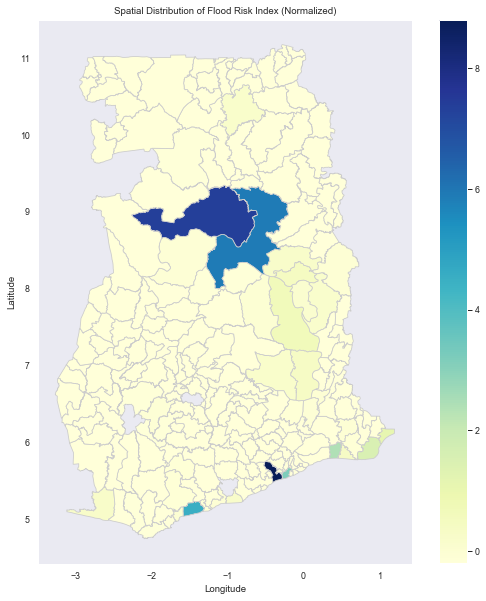
\includegraphics[scale=0.8]{images/01-map.png}
  \end{center}
  \caption{Spatial distribution of final Flood Risk Index}
\end{figure}

As shown in Figure 8.1, the flood-prone districts in Ghana are clustered in the northeast and western regions of the country. The non flood-prone districts of Ghana are all of the surrounding regions. Flood risk experts\footnote{Cloud to Street remote sensing scientists} agree that the map shown in Figure 8.1 above roughly corresponds to their expectations around both flood frequency and social and economic vulnerability. The frequency distribution of these values can be seen in Figure 8.2. \\

\begin{figure}
  \begin{center}
    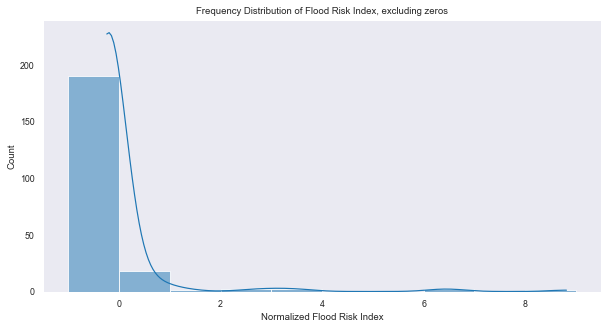
\includegraphics[scale=0.7]{images/02-graph.png}
  \end{center}
  \caption{Frequency distribution of final Flood Risk Index}
\end{figure}

Figure 8.2 illustrates the distribution of the normalized flood risk index values (i.e. the z-score conversion of the raw index values). Each bin of the histogram represents one standard deviation from the mean. From the frequency distribution, we can see that the vast majority of Ghana’s 216 districts fall within 1 standard deviation below the normalized mean of the Flood Risk Index. A small percentage of districts are severely high risk, falling anywhere from 3 to 8 standard deviations above the mean.

\section{Threshold the Flood Risk Index}

\begin{figure}
  \begin{center}
    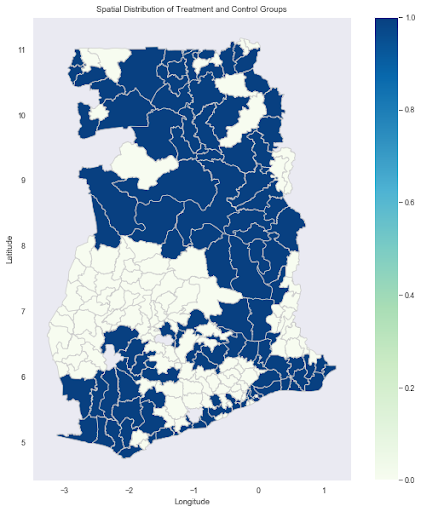
\includegraphics[scale=0.95]{images/03-map.png}
  \end{center}
  \caption{Spatial distribution of treatment-control boundary}
\end{figure}

After all of Ghana’s 216 districts were given a value on the normalized Flood Risk Index, a threshold was set to mark the point beyond which a given district would be labelled ‘flood-prone’ and thus placed into the Treatment Group. Because empirical methods could not be used to identify an appropriate threshold, the threshold was set arbitrarily following the expertise of remote sensing scientists familiar with the flood risk landscape in Ghana.\\

\begin{figure}
  \begin{center}
    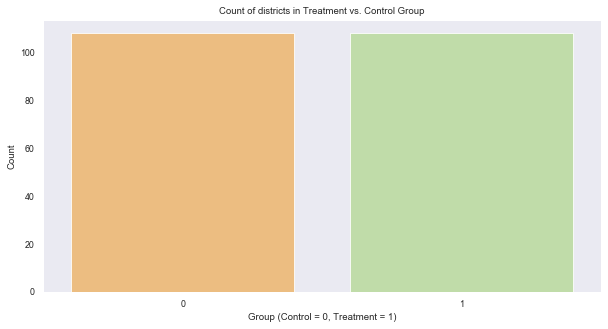
\includegraphics[scale=0.7]{images/04-graph.png}
  \end{center}
  \caption{Frequency distribution of treatment-control boundary}
\end{figure}

The threshold used was the 50th percentile. This meant that the 216 Ghanaian districts which ranked in the top 50 percent of the Flood Risk Index were grouped into Treatment, and all remaining districts (i.e. those in the bottom 50 percent) were grouped into Control. The spatial distribution of treatment and control groups can be seen in Figure 8.3. The map in Figure 8.3 illustrates the spatial distribution of the treatment-control assignment using the 50th percentile threshold. Using this threshold, treatment districts are classified as those in  mid and northern Ghana, as well as southwest Ghana. Control districts are all those surrounding these districts. \\

The number of districts in each group is illustrated in Figure 8.4. Because the threshold was set at the 50th percentile, exactly half of the 216 districts (108 districts) were binned in the treatment and control group each.

\section{Examine parallel trends between treatment and control groups on the outcome variables}

After grouping all of Ghana’s 216 districts into either Treatment or Control, the final step was to examine group means on observable characteristics to determine if there existed parallel trends. As mentioned in earlier sections of this paper, the validity of the Control group as a counterfactual for the Treatment group hinges on the existence of parallel trends between Treatment and Control Groups prior to the start of the program. \\

Parallel trends were examined on two outcome variables of interest:

\begin{itemize}
    \item The average number of total flood-affected people per district, and
    \item The average area of total flood-affected cropland per district.
\end{itemize}

Using line graphs, we are able to see visually that for the 35-year satellite record, parallel trends do not exist in the average number of total flood-affected people per district in the treatment versus control group. These visual trends are shown in Figure 8.5. \\

\begin{figure}
  \begin{center}
    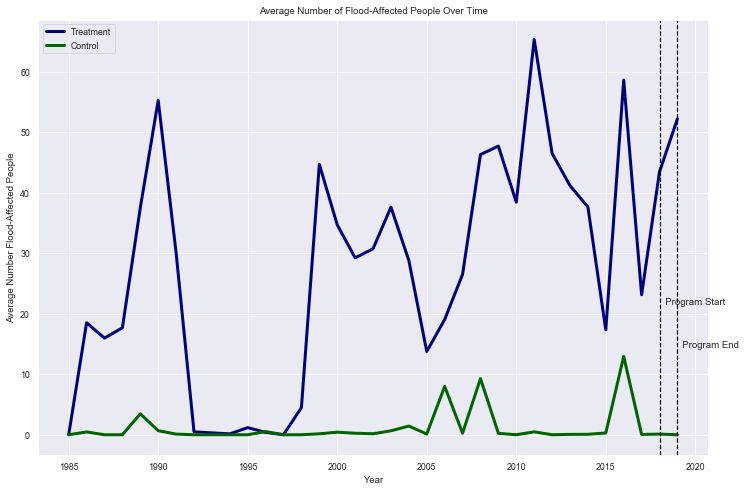
\includegraphics[scale=0.6]{images/05-parallel-trends-population.png}
  \end{center}
  \caption{Visualization of parallel trends test in total flood-affected population outcome variable.}
\end{figure}

\begin{figure}
  \begin{center}
    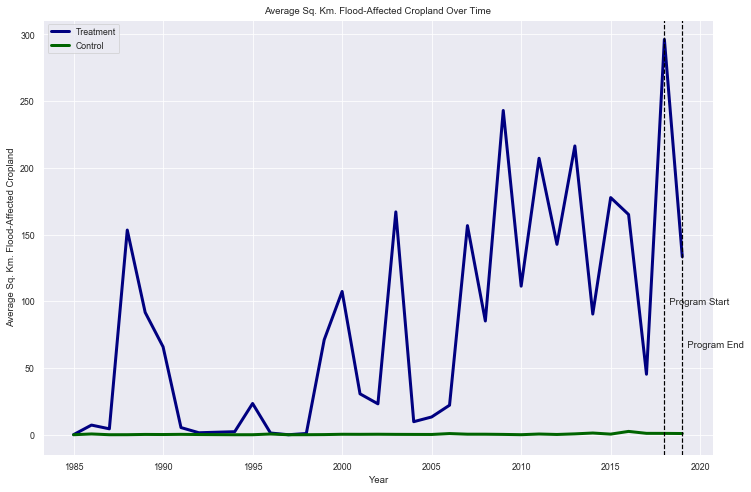
\includegraphics[scale=0.6]{images/06-parallel-trends-cropland.png}
  \end{center}
  \caption{Visualization of parallel trends test in total flood-affected cropland outcome variable.}
\end{figure}

The year-over-year change in the mean flood-affected population over the last 35 years in the satellite record shows a lack of parallel trends between treatment and control group means.

Parallel trends means that the lines in this line graph are parallel, where each line represents the group mean in a given year. When examining the treatment group on average flood-affected population overtime in Figure 8.5, we see that the lines are not parallel in all years prior to the year 2015. From 2015 to 2018, the lines are parallel. 2015 onward, the rates of change from one year to the next are in the correct direction (increase from 2015 to 2016, decrease from 2016 to 2017, and increase from 2017 to 2018). However, the rates of change are not consistent across Treatment and Control groups; in 2016 for example, there was an 1.7 percent increase in average flood affected population for the Treatment group but a 10.6 percent increase for the Control group. When examining the treatment group on average flood-affected cropland overtime in Figure 8.6, we see that the line exhibits a highly cyclical pattern. Meanwhile, the control group on this characteristic has a flat line. The lines are clearly not parallel to one another.

Mathematically, we can confirm this visual pattern of a lack of parallel trends by calculating the slope of the line between each year on the x-axis, using point-slope form:

\[ {m} = ({x_1 - x_2}) / ({y_1 - y_2}) \]

The data shown in Figure 8.5 was used to calculate the slope of each line to mathematically confirm that we do not observe parallel trends. As shown in Figure 8.5 the x-axis pertain to a given year, and the y-axis pertains to the average number of flood affected people in the given year. \\

Thus, (\({x_1 - x_2}\)) pertains to the change in number of years, and (\({y_1 - y_2}\)) pertains to the change in average number of flood-affected people over those number of years. The complete list of slope calculations can be found in Appendix 12.1: Mathematical confirmation of a lack of parallel trends. \\

The lack of parallel trends across these two outcome variables indicates the presence of selection bias in the treatment and control group assignment. This means that using the Flood Risk Index in its current form as the group assignment variable does not allow the control group to serve as a valid counterfactual for the treatment group. Running a double difference estimation on these groups would ultimately not produce an unbiased estimate of the average treatment effect. Several extraneous factors could explain any observed differences in the treatment and control group on food security outcome variables of interest.


\chapter{Discussion}

An unbiased estimate of the average treatment effect could not be derived at this time, for two reasons:

\begin{enumerate}
  \item A lack of annualized, district-level data on food security in Ghana.
  \item A lack of parallel trends between Treatment and Control Groups on the potential outcome variable of interest.
\end{enumerate}

Each challenge is described further in the following sections. Finally, this section provides the equations one would use to derive the double difference estimator in the two challenges above were to be resolved.

\subsection{A lack of annualized, district-level data on food security in Ghana}

Completing this impact evaluation requires annualized, district-level data in Ghana on the primary outcome variable of interest: food security. Traditionally, such data could be obtained using  in-country surveys to collect baseline and endline data. In the absence of the resources required to do this, one could solicit secondary sources for this information. Unfortunately, annualized, district-level data on food security in Ghana was unable to be requisitioned in the time available to conduct this study.

\subsection{A lack of parallel trends between Treatment and Control Groups on the potential outcome variable of interest}

In addition to appropriate data on the outcome variable of interest, completing this impact evaluation also requires a valid counterfactual for the treatment group. In a double difference evaluation, this is established through parallel trends in group means on observable characteristics. The data available to conduct the parallel trends analysis revealed a lack of parallel trends in group means. This could be remedied in some of the following ways:

\begin{enumerate}
  \item Reconstructing the Flood Risk Index to include other components of flood risk. With additional data, one could reconstruct the flood risk index to define flood risk differently or more comprehensively.
  \item Constructing a counterfactual with a "synthetic" method.
\end{enumerate}

\subsection{Double-Difference Estimation}

In the future, if one is able to resolve the two challenges above, one could proceed with deriving the double difference estimate of the ATE. The following section explains how this would be done. In general, in the absence of selection bias and after ensuring parallel trends, one could derive the double difference estimator using a multivariate OLS regression:

\[ Y = alpha + beta (treatment) + gamma (post) + delta (treatment * post) + e \]

In this formula, the variables `treatment` and `post` are boolean, where 1 indicates the Treatment group or post-period respectively, and 0 indicates the Control group or the pre-period respectively. The dependent variable `Y` refers to the outcome variable of interest: district or household-level food security. The term `e` represents the error term.\\

Each coefficient on the independent variables represents the program’s impact on the pre-period control, pre-period treatment, post-period control and post-period treatment groups relative to the other groups, respectively. The coefficients alpha, beta, gamma and delta refer to the impact of the program on the pre-period control, pre-period treatment, post-period control and post-period treatment groups relative to the other groups, respectively.\\

The `delta` coefficient in the OLS regression is our unbiased estimate of the average treatment effect. `delta` is also equivalent to the following, which illustrates more clearly the double difference intuition:

\[ delta = (T_{post} - T_{pre}) - (C_{post} - C_{pre}) \]

This formula will compute a value for delta that is equivalent to the value of delta in the OLS regression, but it more intuitively illustrates what the double difference estimator is. The double difference estimator, as seen here, is the difference between treatment and control group means before and after the program. It is important to note that the coefficient delta only provides an unbiased estimator of the ATE if the identifying assumption of parallel trends is satisfied. Otherwise the coefficient is at best a measure of correlation between the program and the outcome variable of interest.

\chapter{Extensions}

This section outlines extensions to the research that could be explored in the future.

\section{The FIS as a pre-flood early warning platform}

The current quasi-experimental design of the study examines the efficacy of the FIS as a post-flood, aid targeting mechanism. However, NADMO officials that use the FIS have indicated their interest in using the FIS as a principal component of a redesigned internal process in which satellite-based flood information informs long-term flood preparedness. Part of this effort could involve preventative relocation, an increasingly popular climate change adaptation strategy, in which civilians living in floodplains are moved out of the floodplain in order to reduce loss of life.\\

In its current form the FIS has supported NADMO primarily as a post-flood aid targeting platform. In future years of the program, however, if NADMO begins to use the FIS in any pre-flood capacity (for preventative relocation or otherwise), the damage data readily available through satellites could serve as an appropriate outcome variable of interest.



\printbibliography

% \appendix
% \chapter{More Monticello Candidates}

\end{document}
